% This file is auto-generated using the function figure1 in
% figures/figure1.m with frakb = \frac{\sqrt{5} + 5}{2}\Z_F and B = 36
% and parameters:
% scale = 0.9000, max_grid = 12.0000, min_grid = -2.0000
% margin = 1.0000, min_shadows = 3, radius = 0.0500
\begin{figure}
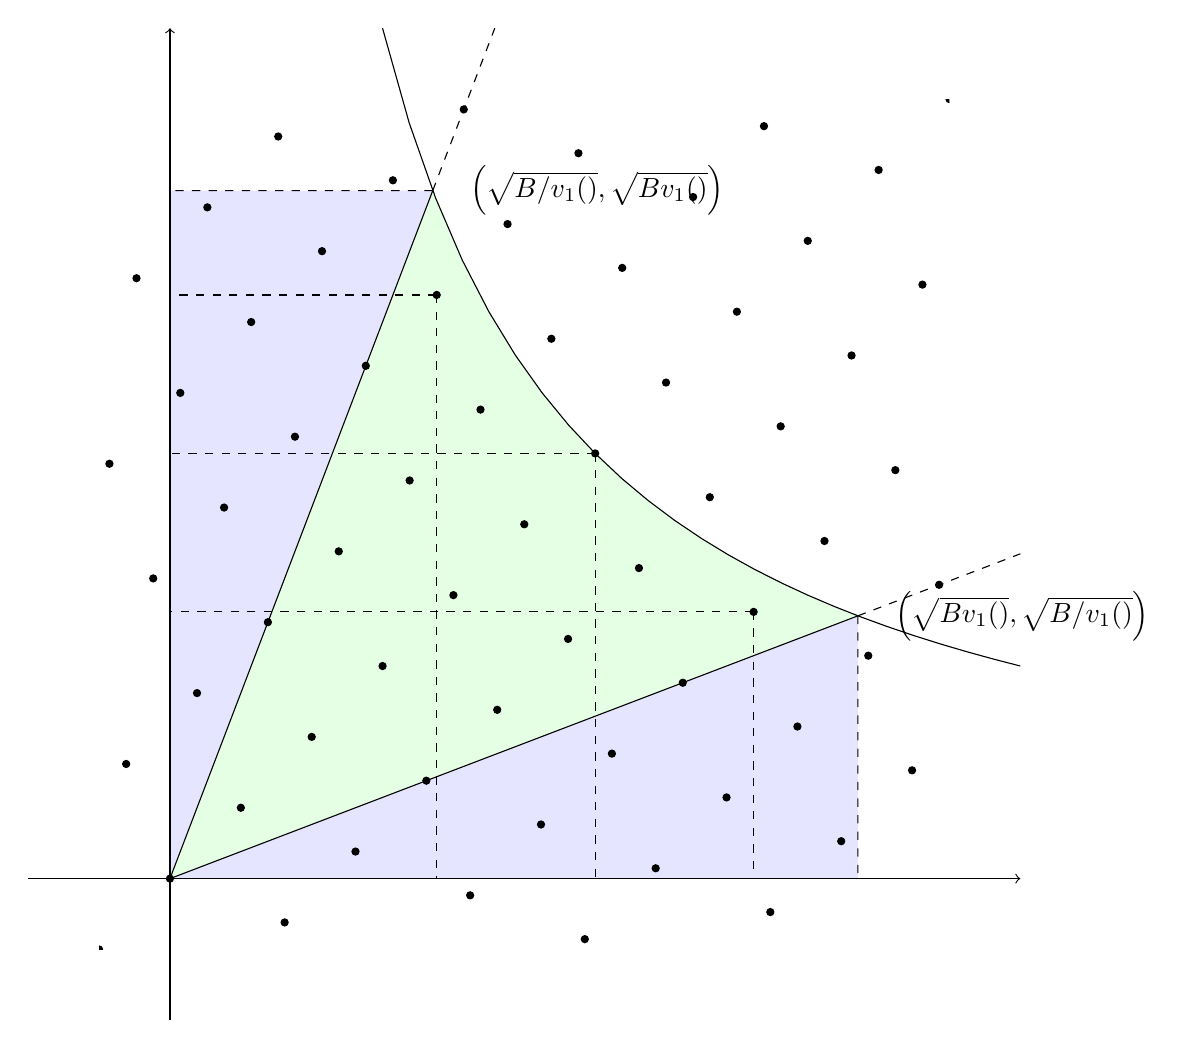
\begin{tikzpicture}[scale=0.9000]
%Vertices of Shintani cone
\def\xA{9.7082}
\def\yA{3.7082}
\draw node (A) at (\xA, \yA) {};
\draw node[right] at (A) {$\quad \left(\sqrt{Bv_1(\eps)},\sqrt{B/v_1(\eps)}\right)$};
\draw node (B) at (\yA, \xA) {};
\draw node[right] at (B) {$\quad \left(\sqrt{B/v_1(\eps)},\sqrt{Bv_1(\eps)}\right)$};
%Fill
\fill [blue!10] (0,0) -- (A.center) -- (\xA, 0);
\fill [blue!10] (0,0) -- (B.center) -- (0, \xA);
\fill [green!10] (0,0) -- (B.center)
plot [domain=\yA:\xA] (\x,36/\x)
-- (A.center) -- (0,0);
%Axes
\draw [->] (0,-2.0000) -- (0,12.0000);
\draw [->] (-2.0000,0) -- (12.0000,0);
%Norm bound
\draw [domain=3.0000:12.0000] plot (\x,36/\x);
%Shintani axes
\draw (0,0) -- (A.center);
\draw [dashed] (A.center) -- (12.0000, 4.5836);
\draw (0,0) -- (B.center);
\draw [dashed] (B.center) -- (4.5836, 12.0000);
%Projections
\draw [dashed] (A.center) -- (\xA, 0);
\draw [dashed] (B.center) -- (0, \xA);
%Lattice points
{\clip (-1.0000,-1.0000) rectangle (11.0000,11.0000);
\def\xx{{-1.0000}}
\def\yy{{-1.0000}}
\draw[fill] ({\xx},{\yy}) circle (0.0500);
\def\xx{{0.0000}}
\def\yy{{0.0000}}
\draw[fill] ({\xx},{\yy}) circle (0.0500);
\def\xx{{1.6180}}
\def\yy{{-0.6180}}
\draw[fill] ({\xx},{\yy}) circle (0.0500);
\def\xx{{-0.6180}}
\def\yy{{1.6180}}
\draw[fill] ({\xx},{\yy}) circle (0.0500);
\def\xx{{1.0000}}
\def\yy{{1.0000}}
\draw[fill] ({\xx},{\yy}) circle (0.0500);
\def\xx{{2.6180}}
\def\yy{{0.3820}}
\draw[fill] ({\xx},{\yy}) circle (0.0500);
\def\xx{{0.3820}}
\def\yy{{2.6180}}
\draw[fill] ({\xx},{\yy}) circle (0.0500);
\def\xx{{4.2361}}
\def\yy{{-0.2361}}
\draw[fill] ({\xx},{\yy}) circle (0.0500);
\def\xx{{2.0000}}
\def\yy{{2.0000}}
\draw[fill] ({\xx},{\yy}) circle (0.0500);
\def\xx{{-0.2361}}
\def\yy{{4.2361}}
\draw[fill] ({\xx},{\yy}) circle (0.0500);
\def\xx{{5.8541}}
\def\yy{{-0.8541}}
\draw[fill] ({\xx},{\yy}) circle (0.0500);
\def\xx{{3.6180}}
\def\yy{{1.3820}}
\draw[fill] ({\xx},{\yy}) circle (0.0500);
\def\xx{{1.3820}}
\def\yy{{3.6180}}
\draw[fill] ({\xx},{\yy}) circle (0.0500);
\def\xx{{-0.8541}}
\def\yy{{5.8541}}
\draw[fill] ({\xx},{\yy}) circle (0.0500);
\def\xx{{5.2361}}
\def\yy{{0.7639}}
\draw[fill] ({\xx},{\yy}) circle (0.0500);
\def\xx{{3.0000}}
\def\yy{{3.0000}}
\draw[fill] ({\xx},{\yy}) circle (0.0500);
\def\xx{{0.7639}}
\def\yy{{5.2361}}
\draw[fill] ({\xx},{\yy}) circle (0.0500);
\def\xx{{6.8541}}
\def\yy{{0.1459}}
\draw[fill] ({\xx},{\yy}) circle (0.0500);
\def\xx{{4.6180}}
\def\yy{{2.3820}}
\draw[fill] ({\xx},{\yy}) circle (0.0500);
\def\xx{{2.3820}}
\def\yy{{4.6180}}
\draw[fill] ({\xx},{\yy}) circle (0.0500);
\def\xx{{0.1459}}
\def\yy{{6.8541}}
\draw[fill] ({\xx},{\yy}) circle (0.0500);
\def\xx{{8.4721}}
\def\yy{{-0.4721}}
\draw[fill] ({\xx},{\yy}) circle (0.0500);
\def\xx{{6.2361}}
\def\yy{{1.7639}}
\draw[fill] ({\xx},{\yy}) circle (0.0500);
\def\xx{{4.0000}}
\def\yy{{4.0000}}
\draw[fill] ({\xx},{\yy}) circle (0.0500);
\def\xx{{1.7639}}
\def\yy{{6.2361}}
\draw[fill] ({\xx},{\yy}) circle (0.0500);
\def\xx{{-0.4721}}
\def\yy{{8.4721}}
\draw[fill] ({\xx},{\yy}) circle (0.0500);
\def\xx{{7.8541}}
\def\yy{{1.1459}}
\draw[fill] ({\xx},{\yy}) circle (0.0500);
\def\xx{{5.6180}}
\def\yy{{3.3820}}
\draw[fill] ({\xx},{\yy}) circle (0.0500);
\def\xx{{3.3820}}
\def\yy{{5.6180}}
\draw[fill] ({\xx},{\yy}) circle (0.0500);
\def\xx{{1.1459}}
\def\yy{{7.8541}}
\draw[fill] ({\xx},{\yy}) circle (0.0500);
\def\xx{{9.4721}}
\def\yy{{0.5279}}
\draw[fill] ({\xx},{\yy}) circle (0.0500);
\def\xx{{7.2361}}
\def\yy{{2.7639}}
\draw[fill] ({\xx},{\yy}) circle (0.0500);
\def\xx{{5.0000}}
\def\yy{{5.0000}}
\draw[fill] ({\xx},{\yy}) circle (0.0500);
\def\xx{{2.7639}}
\def\yy{{7.2361}}
\draw[fill] ({\xx},{\yy}) circle (0.0500);
\def\xx{{0.5279}}
\def\yy{{9.4721}}
\draw[fill] ({\xx},{\yy}) circle (0.0500);
\def\xx{{8.8541}}
\def\yy{{2.1459}}
\draw[fill] ({\xx},{\yy}) circle (0.0500);
\def\xx{{6.6180}}
\def\yy{{4.3820}}
\draw[fill] ({\xx},{\yy}) circle (0.0500);
\def\xx{{4.3820}}
\def\yy{{6.6180}}
\draw[fill] ({\xx},{\yy}) circle (0.0500);
\def\xx{{2.1459}}
\def\yy{{8.8541}}
\draw[fill] ({\xx},{\yy}) circle (0.0500);
\def\xx{{10.4721}}
\def\yy{{1.5279}}
\draw[fill] ({\xx},{\yy}) circle (0.0500);
\def\xx{{8.2361}}
\def\yy{{3.7639}}
\draw[fill] ({\xx},{\yy}) circle (0.0500);
\def\xx{{6.0000}}
\def\yy{{6.0000}}
\draw[fill] ({\xx},{\yy}) circle (0.0500);
\def\xx{{3.7639}}
\def\yy{{8.2361}}
\draw[fill] ({\xx},{\yy}) circle (0.0500);
\def\xx{{1.5279}}
\def\yy{{10.4721}}
\draw[fill] ({\xx},{\yy}) circle (0.0500);
\def\xx{{9.8541}}
\def\yy{{3.1459}}
\draw[fill] ({\xx},{\yy}) circle (0.0500);
\def\xx{{7.6180}}
\def\yy{{5.3820}}
\draw[fill] ({\xx},{\yy}) circle (0.0500);
\def\xx{{5.3820}}
\def\yy{{7.6180}}
\draw[fill] ({\xx},{\yy}) circle (0.0500);
\def\xx{{3.1459}}
\def\yy{{9.8541}}
\draw[fill] ({\xx},{\yy}) circle (0.0500);
\def\xx{{9.2361}}
\def\yy{{4.7639}}
\draw[fill] ({\xx},{\yy}) circle (0.0500);
\def\xx{{7.0000}}
\def\yy{{7.0000}}
\draw[fill] ({\xx},{\yy}) circle (0.0500);
\def\xx{{4.7639}}
\def\yy{{9.2361}}
\draw[fill] ({\xx},{\yy}) circle (0.0500);
\def\xx{{10.8541}}
\def\yy{{4.1459}}
\draw[fill] ({\xx},{\yy}) circle (0.0500);
\def\xx{{8.6180}}
\def\yy{{6.3820}}
\draw[fill] ({\xx},{\yy}) circle (0.0500);
\def\xx{{6.3820}}
\def\yy{{8.6180}}
\draw[fill] ({\xx},{\yy}) circle (0.0500);
\def\xx{{4.1459}}
\def\yy{{10.8541}}
\draw[fill] ({\xx},{\yy}) circle (0.0500);
\def\xx{{10.2361}}
\def\yy{{5.7639}}
\draw[fill] ({\xx},{\yy}) circle (0.0500);
\def\xx{{8.0000}}
\def\yy{{8.0000}}
\draw[fill] ({\xx},{\yy}) circle (0.0500);
\def\xx{{5.7639}}
\def\yy{{10.2361}}
\draw[fill] ({\xx},{\yy}) circle (0.0500);
\def\xx{{9.6180}}
\def\yy{{7.3820}}
\draw[fill] ({\xx},{\yy}) circle (0.0500);
\def\xx{{7.3820}}
\def\yy{{9.6180}}
\draw[fill] ({\xx},{\yy}) circle (0.0500);
\def\xx{{9.0000}}
\def\yy{{9.0000}}
\draw[fill] ({\xx},{\yy}) circle (0.0500);
\def\xx{{10.6180}}
\def\yy{{8.3820}}
\draw[fill] ({\xx},{\yy}) circle (0.0500);
\def\xx{{8.3820}}
\def\yy{{10.6180}}
\draw[fill] ({\xx},{\yy}) circle (0.0500);
\def\xx{{10.0000}}
\def\yy{{10.0000}}
\draw[fill] ({\xx},{\yy}) circle (0.0500);
\def\xx{{11.0000}}
\def\yy{{11.0000}}
\draw[fill] ({\xx},{\yy}) circle (0.0500);
}
%Draw three "shadows"
\def\xx{{6.0000}}
\def\yy{{6.0000}}
\draw [dashed] (\xx,\yy) -- (\xx,0);
\draw [dashed] (\xx,\yy) -- (0,\yy);
\def\xx{{8.2361}}
\def\yy{{3.7639}}
\draw [dashed] (\xx,\yy) -- (\xx,0);
\draw [dashed] (\xx,\yy) -- (0,\yy);
\def\xx{{3.7639}}
\def\yy{{8.2361}}
\draw [dashed] (\xx,\yy) -- (\xx,0);
\draw [dashed] (\xx,\yy) -- (0,\yy);
\end{tikzpicture}
\caption{The sets $\FunDomain{\frakb'}{B}$ and $\FunDomShadow{\frakb'}{B}$ for $F = \Q(\sqrt{5})$, $\frakb = \frac{\sqrt{5} + 5}{2}\Z_F$ (so that $\frakb' = \Z_F$), and $B=36$. The set $\FunDomain{\frakb'}{B}$ consists of lattice points in the green region, and the set $\FunDomShadow{\frakb'}{B}$ consists of the points in $\FunDomain{\frakb'}{B}$ as well as the points in the blue region.}
\label{fig:shadow}
\end{figure}
